\section{Results and Measurements}
\label{sec:results}

Tiny Tapeout 2 chips were received in October 2023, 11 months after the chips were submitted for manufacture on the Efabless chipIgnite 2211Q shuttle.
The chips were tested for the first time on a public livestream~\cite{siliconalive}.
During this testing the chain was validated and a small number of the designs were demonstrated to be working.
In further testing following the livestream another 30 designs were tested and shown to be working.

\begin{figure}[!t]
\centering
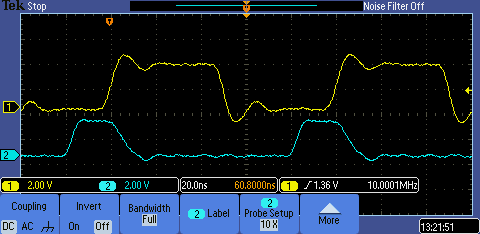
\includegraphics[width=\columnwidth]{./Figs/tt02_clock_out.png}
\caption{Measurement from Tiny Tapeout 2 silicon, with input clock in yellow and the distorted output clock in blue.}
\label{fig:TT02_clock_out}
\end{figure}

After measuring the clock asymmetry (Fig.~\ref{fig:TT02_clock_out}) and maximum frequency it was decided to run the production boards with a \qty{20}{\MHz} oscillator, resulting in a \qty{10}{\MHz} scan chain clock and a \qty{5}{\kHz} IO update rate in order to maximize stability.

Some Tiny Tapeout 2 designs did not function as expected; in most cases this was determineted to be due to faults in the submitted design.

Of the designs submitted 82 used the Verilog HDL, 64 were created using the Wokwi graphical editor, and six used alternative HDLs including VHDL, Amaranth~\cite{amaranth}, and Chisel~\cite{chisel}.

Some of the designs created using Wokwi using combinational logic in clock paths (Fig.~\ref{fig:failed_design_comb_logic}) worked in simulation but failed in hardware.
This was determinted to be due to the lack of timing data in the simulation, and wasn not detected by STA because the clock paths were not known. A detailed analysis on these failures has yet to be carried out.

\begin{figure}[!t]
\centering
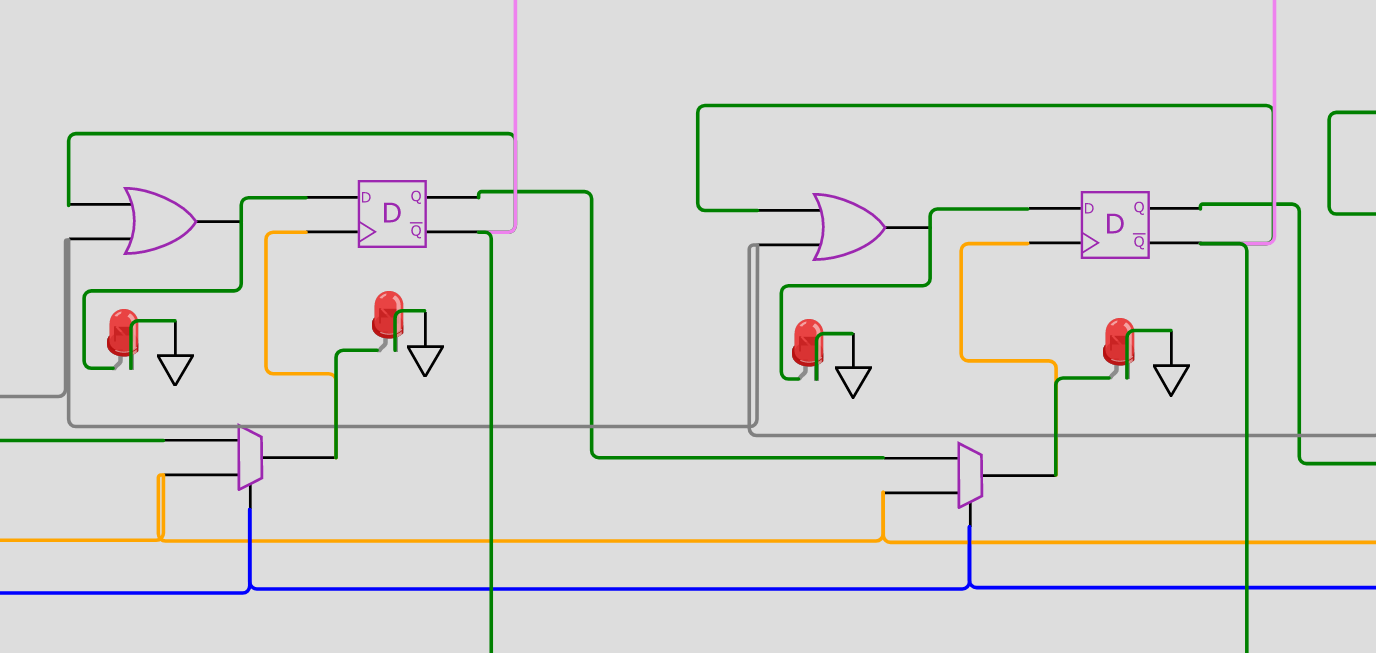
\includegraphics[width=\columnwidth]{./Figs/wokwi mux clock logic.png}
\caption{Combinational logic in the clock path of one of the failed designs.}
\label{fig:failed_design_comb_logic}
\end{figure}

At the time of writing PCBs are in production and are expected to ship to customers by the end of January 2024.

Silicon from Tiny Tapeout 3 production was received in January 2024. The updated scan chain design shows a more symmetric output clock at the end of the chain (Fig.~\ref{fig:TT03_silicon_measurement}). The improved clock symmetry will allow for the use of a faster scan chain clock, resulting in a faster update frequency.

\begin{figure}[!t]
\centering
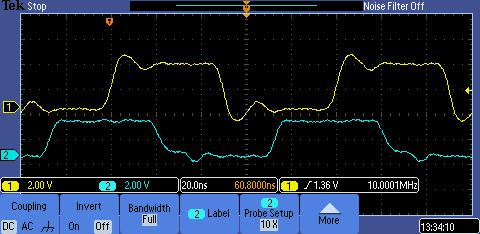
\includegraphics[width=\columnwidth]{./Figs/tt03_clock_out.png}
\caption{Measurement from Tiny Tapeout 3 silicon.}
\label{fig:TT03_silicon_measurement}
\end{figure}

Some Tiny Tapeout 3.5 designs have already been validated, including a VGA clock project (Fig.~\ref{fig:VGA_clock_design_TT03_5_silicon}) which takes advantage of the new higher speed IO.

The overhead of multiplexing multiple tiles makes power consumption of the infrastructure only a minor concern at this point. No direct comparison of the power consumption impact of the multiplexer over the previous scan chain architecture is available at the time of writing. The motivation of the multiplexer approach, however, was to substantially increase the bandwidth of the IOs.

After Tiny Tapeout 4 silicon was received and tested, the worst round trip latency was measured to be \qty{20}{\ns} as shown in Fig~\ref{fig:round_trip_latency_rising_edge} and \ref{fig:round_trip_latency_falling_edge}.

\begin{figure}[!t]
\centering
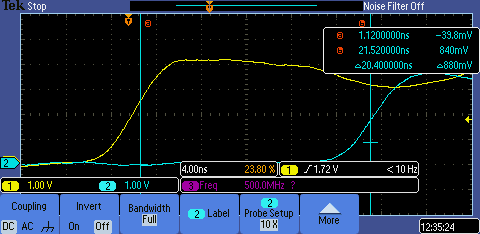
\includegraphics[width=\columnwidth]{./Figs/tt3p5 rising latency.PNG}
\caption{The Tiny Tapeout 3.5 round trip latency on a rising edge, measured at about \qty{20}{\ns}.}
\label{fig:round_trip_latency_rising_edge}
\end{figure}

\begin{figure}[!t]
\centering
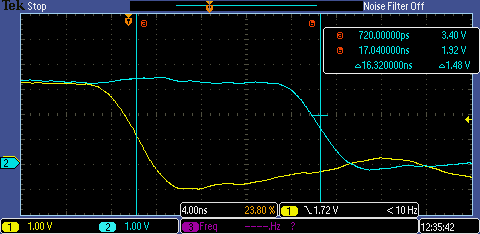
\includegraphics[width=\columnwidth]{./Figs/tt3p5 falling latency.PNG}
\caption{The Tiny Tapeout 3.5 round trip latency on a falling edge, measured at about \qty{16}{\ns}.}
\label{fig:round_trip_latency_falling_edge}
\end{figure}

\begin{figure}[!t]
\centering
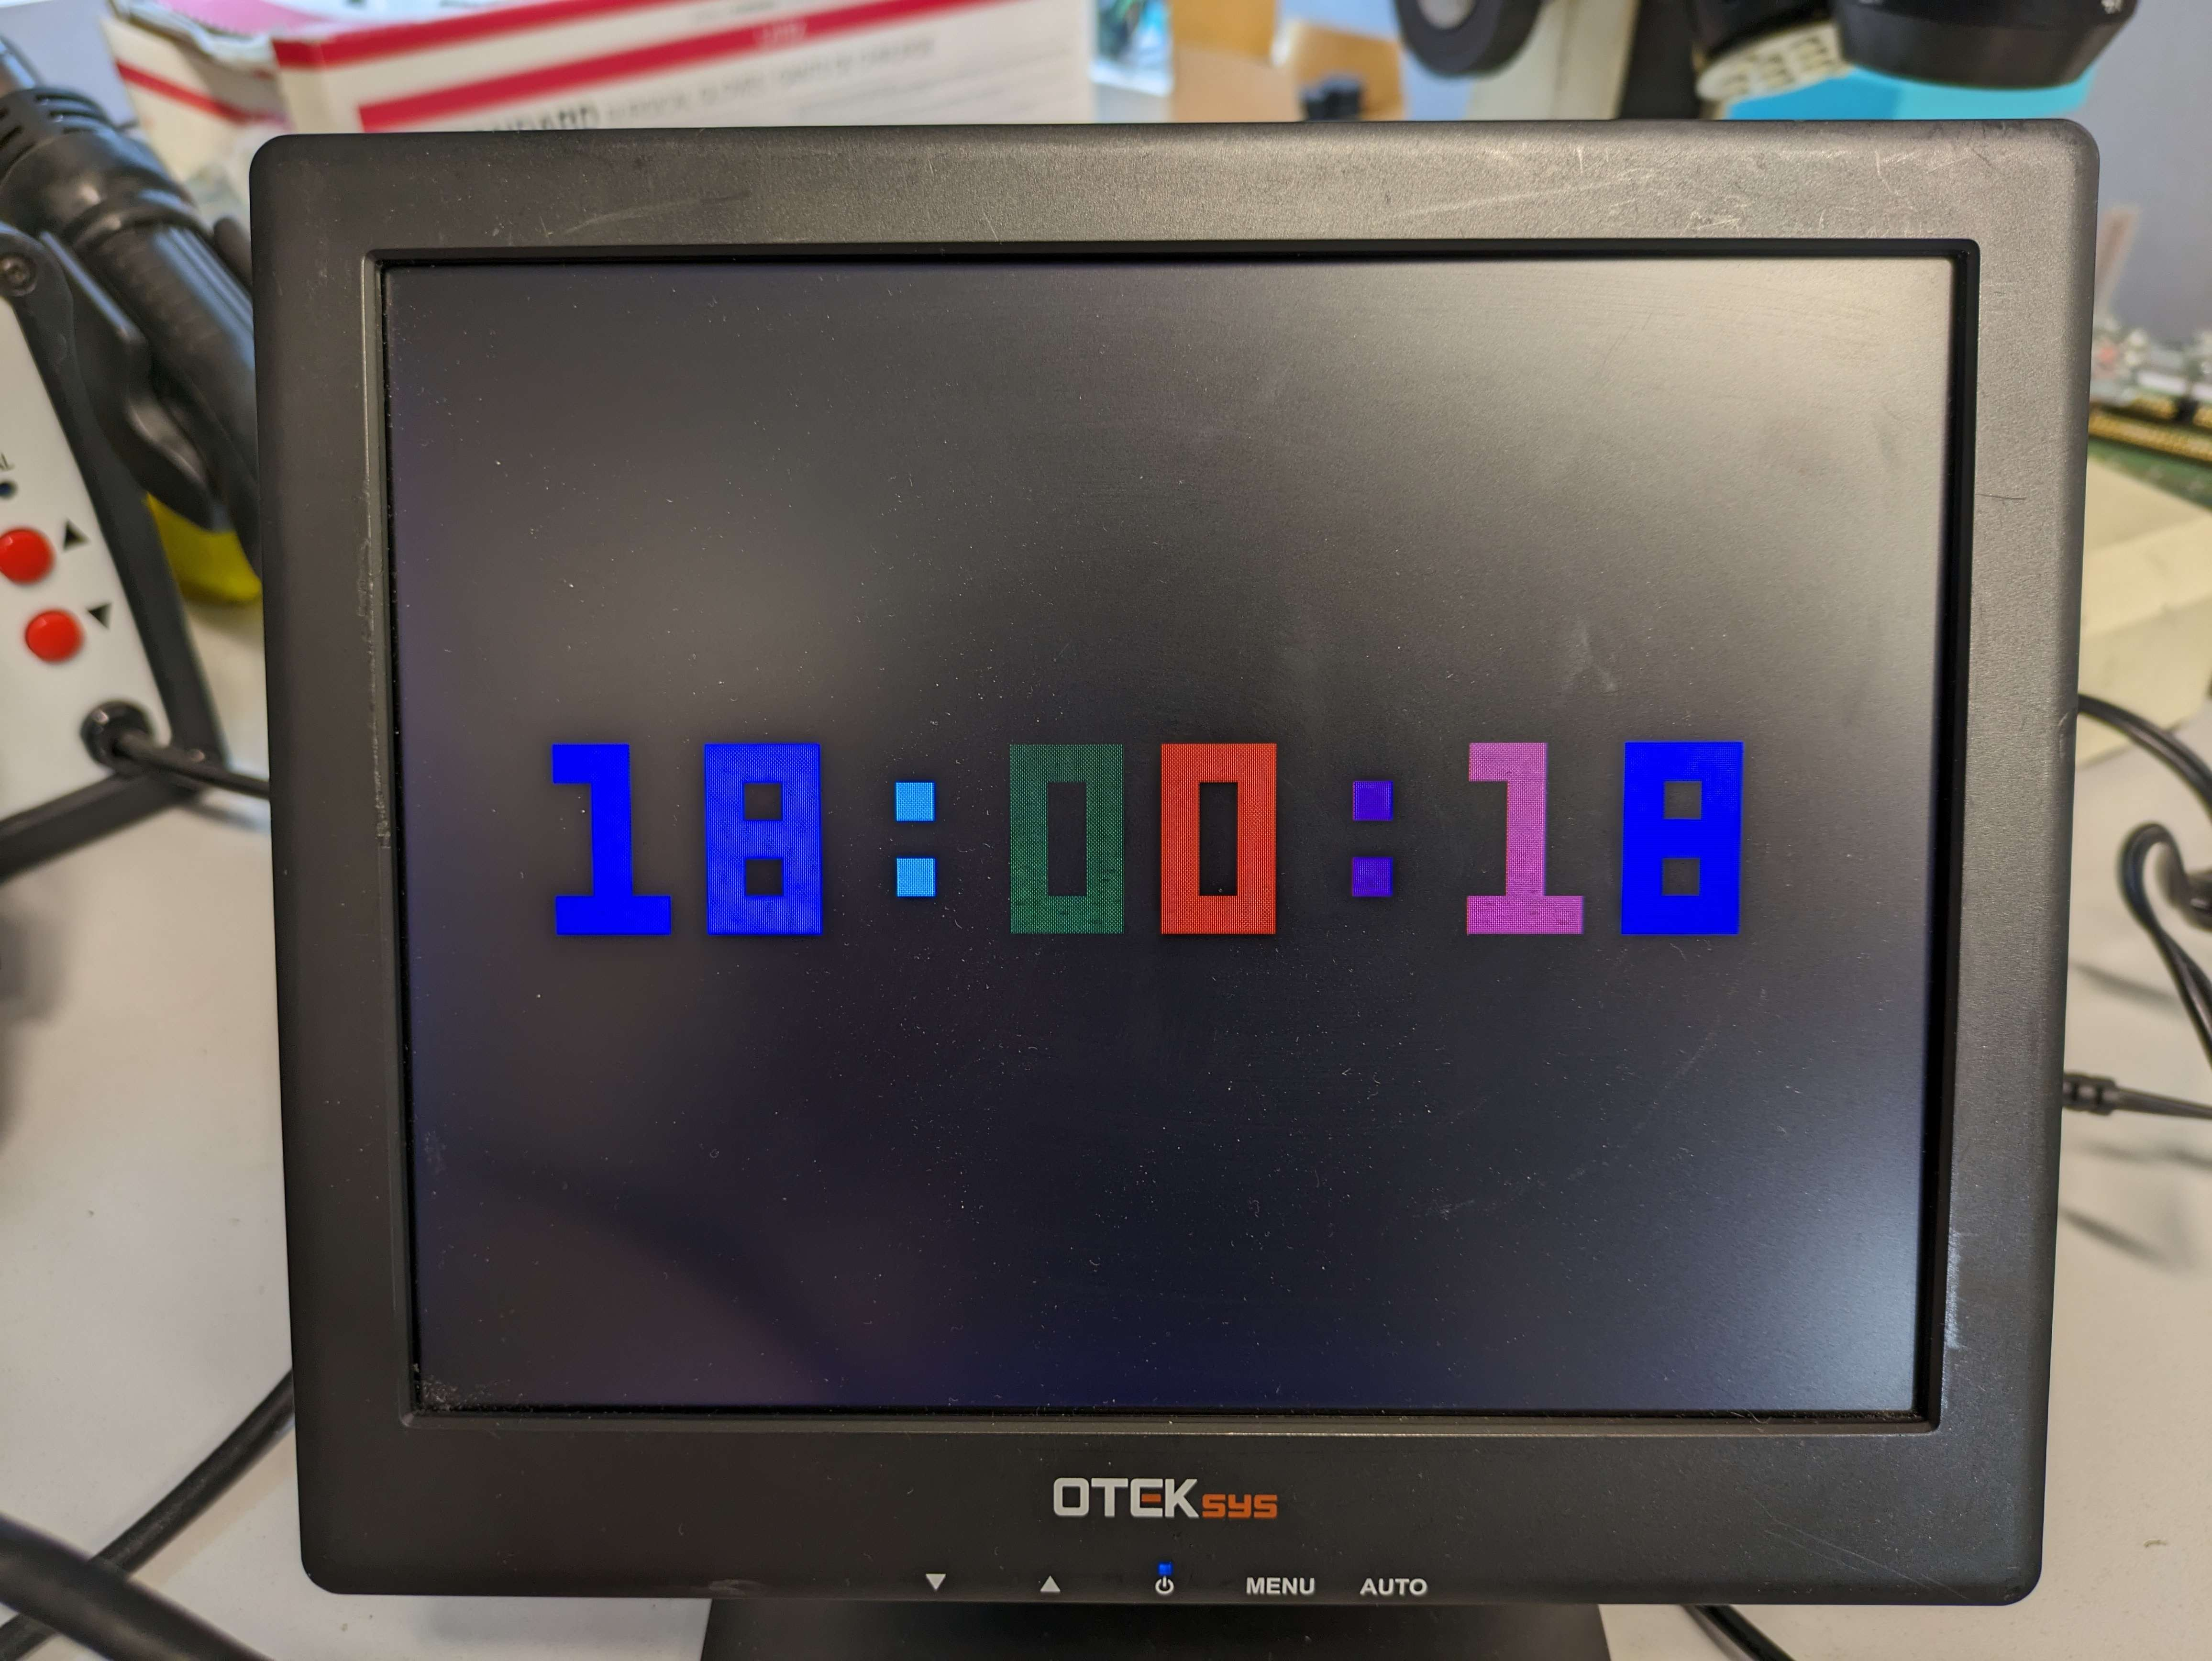
\includegraphics[width=\columnwidth]{./Figs/tt3p5 vga clock.jpg}
\caption{A VGA clock design running on Tiny Tapeout 3.5 silicon.}
\label{fig:VGA_clock_design_TT03_5_silicon}
\end{figure}
